\chapter{基于模型融合的分心驾驶行为检测系统}

\section{引言}

本文主要是结合第三章以及第四章的内容,设计一个自然场景下的分心驾驶行为检测系统,用以对自然场景下驾驶员分心驾驶行为检测的模拟。本章首先介绍了软件相关环境配置,然后详细介绍了分心驾驶行为检测系统的系统方案和之遥的相关步骤及主要参数的选择,最后对系统进行了检测测试。

\section{系统软件环境}

(1)	软件环境

本文选择的开发环境是考虑到可移植特性的基础上,选择具有跨平台特性的的软件开发架构,在Windows和Linux及其开发板Jetson等开发板上,都可通过很小的调整而直接使用。

\begin{table}[!ht]
	\caption{系统依赖软件包及其对应版本}
	\label{表5.1}
	\renewcommand{\arraystretch}{1.5}
	\centering
	\begin{tabular}{p{4.5cm}<{\centering}|p{4.5cm}<{\centering}}
		\bottomrule
		依赖软件包         & 版本号      \\ \hline
		Python        & 3.8.10   \\
		PyTorch       & 1.7.1    \\
		Numpy         & 1.20.2   \\
		PyQt5         & 5.9.2    \\
		Torchvision   & 0.8.2    \\
		OpenCv-Python & 4.5.1.48 \\
		Vit-PyTorch   & 0.26.7   \\ \bottomrule
	\end{tabular}
\end{table}


所需的软件包环境及其版本问题如表\ref{表5.1}所示。以PyTorch深度学习框架为核心,搭配OpenCV的数据处理采集部分,在PyQt的UI交互平台实现系统的整体交互,完成分心驾驶行为检测的模拟。

(2)	RViT模型训练

作为分心驾驶行为检测系统的主要核心不可替代部分,可靠的网络模型能够提升系统整体的性能。准确率高、可靠性强能够在复杂的条件下可以长时间稳定运行,是网络工程化的应用标准。

\begin{figure}[!ht]
	\centering
	\includegraphics[height=8.18cm ,width=13.59cm]{figures/图5.1.eps}
	\caption{分心驾驶行为AUDC2数据集分布详情}\label{5.1}
\end{figure}


RViT网络作为Transformer网络的变种,继承了其特性,为了发挥优良的特性。使用迁移学习,在大型分类数据集ImagNet上进行预训练调优模型,再通过分心驾驶行为数据集AUCD2的微调,使得模型具有更强的鲁棒性。


由于数据集AUDC2的数据情况分布如图\ref{5.1}所示,分类类别中有样本分布不均匀的情况,即样本类别数量之间差距过大,出现第四章论述的样本失衡问题(多数样本类别对少数样本类别在角特征空间出现挤压问题)。使用第四章孤立中心损失函数ICL对数据集ACUD2样本进行抗挤压微调训练。

预训练和训练过程与第三章实验设置相同,将图像进行翻转、随机裁剪等增强方法,最后输入RViT网络,使用ICL进行监督学习,详细配置见3.3.1小结。

\begin{figure}[!ht]
	\centering
	\includegraphics[height=8.43cm ,width=11.86cm]{figures/图5.2.eps}
	\caption{分心驾驶行为检测系统UI交互界面}\label{5.2}
\end{figure}

(3)	UI界面

为了交互的便利,本文的分心驾驶行为检测技术设计交互界面进行工程模拟,如图\ref{5.2}所示,标记1为获取驾驶行为的图像框;标记2的10各进度条,表示分心驾驶行为属于该类别的概率;标记3为分心驾驶行为检测的预测值;点击“打开”获取分心驾驶行为图像,点击“运行”怎系统开始工作,输出预测结果。


\section{系统设计方案}

一个完整的分心驾驶行为检测系统包括图像预处理、驾驶行为特征提取和驾驶行为检测分类等等,本文旨在将融合模型RViT在工程中的应用进行相应的模拟实现,方便未来在不同的使用场景中进行研究,因此忽略一些特殊的使用条件的限制。在视觉任务中,无所不在的图像噪声是影响视觉任务的一个重要因素,因此图像质量预处理环节是必要的,并且认定图像采集传感器采集到的图像不含超强光,只含有图像噪声的影响。

\begin{figure}[!ht]
	\centering
	\includegraphics[height=6.8cm ,width=11.31cm]{figures/图5.3.eps}
	\caption{AUCD2测试集含噪声图像识别准确率变化}\label{5.3}
\end{figure}

图像噪声强度估计,根据第二章内容,对分心驾驶AUCD2测试集图像添加不同噪声强度的噪声,使用预训练好的RViT网络模型对含有噪声的AUCD2测试集图像进行识别,识别统计结果如图\ref{5.3}所示。可以明确的观察到,随着噪声轻度$\sigma$的增强,分心类别的识别准确率在急剧下降,当噪声强度超过$\sigma=15$时,识别准确率已不足73\%,此时人眼以经无法分辨图像内容。因此,图像噪声过大严重影响模型的性能发挥,去噪是必不可少的环节。


当噪声强度为$\sigma<4$时,模型识别准确率高于98.73\%;当噪声强度$\sigma=6$时,模型识别准确率为95.43\%,相比较于噪声强度$\sigma=4$时下降了3.3\%。当噪声强度$\sigma>9$时,识别率急剧下降到90\%以下,下降效果明显。因此,综合考虑,选择噪声强度$\sigma=3$的阈值,作为图像噪声去噪与否的判决条件。

本文设计的工程模拟分心驾驶行为检测系统如图\ref{5.4}所示,首先从图像采集传感器采集图像,进行图像质量处理。根据第二章图像预处理内容,分为图像噪声强度检测和去噪两部分,图像噪声强度阈值设置为$\sigma=4$,如果噪声强度$\sigma<4$,则图像噪声过多,需要使用高斯滤波技术去噪处理;否则不对图像进行任何处理,直接进行下一步操作。


\begin{figure}[!ht]
	\centering
	\includegraphics[height=10.84cm ,width=5.78cm]{figures/图5.4.eps}
	\caption{分心驾驶行为检测系统主体流程图}\label{5.4}
\end{figure}

其次,对预处理之后的图像送入到预训练好的RViT网络,进行十分类的驾驶行为检测,给出每一类驾驶行为的预测结果,在UI界面展示出最高概率类别判定结果,并进行交互展示。


\section{系统测试}

在Windows系统平台中运行分心驾驶行为检测模拟系统,验证检测效果。如图\ref{5.5}所示,分心驾驶的个别测试效果实例,在左边框图中能够不断的更新驾驶行为图像,根据图像的驾驶行为类别,右边守时能够给出当前图像的每类类别概率值,相应的在正下方显示当前的类别判定,即最终的判定结果为当前概率的最大值类别。具体程序流程如下所示:

\begin{figure}[!ht]
	\centering
	\includegraphics[height=13.97cm ,width=12.87cm]{figures/图5.5.2.eps}
	\caption{分心驾驶行为检测系统主体流程图}\label{5.5}
\end{figure}


1、 OpenCV-Python驱动图像采集传感器获取图像信息;

2、 对获取到的图像信息进行噪声强度估计,并按照噪声强度的不同执行不同的后续操作,即噪声强度$\sigma<4$的图像进行裁剪为(224,224)的尺寸,直接进行第4步骤RViT网络鉴别,对噪声强度$\sigma>4$的图像,传输至第三步骤,进行高斯滤波去噪技术,去除图像的高斯白噪声;

3、 所含噪声图像,在此步骤将被进行去噪处理,将去除噪声之后的图像传输至第4步骤,进行分心驾驶行为检测识别;

4、 将输入到RViT网络中的图像进行十种类别概率的预测,依次将输出的概率在图\ref{5.5}的右边显示出来,并且选择最高概率所在类别,为当前识别图像的驾驶行为分类。


选择测试者,做出不同类别的驾驶行为,采集相应的图像、系统鉴别、给出相应的鉴别结果并实时的显示出来。

对于分心驾驶行为检测的算法研究,使用工程模拟系统,通过了测试,达到了实时反馈信息的效果。模拟噪声的环境效果,设定场景,检测了去噪的效果后的鉴别效果,同样达到了设计的目的,能够有效的鉴别分心驾驶的行为。


\section{本章小节}

本章是在前面第三章融合RViT模型和第四章孤立中心损失函数ICL的基础上,设计了分心驾驶行为检测的工程模拟系统,进行工程验证模拟实验。在此基础上,考虑到图像采集设备和外界环境的影响,添加了第二章的图像质量处理模块,对图像噪声进行噪声估计,考虑到图像噪声来源大多数以高斯白噪声为主,因此选择了成熟的高斯滤波技术进行噪声去除操作。


本章详细阐述了,使用到的工程模拟环境的需求、系统设计方案。在此基础上,统计分析了噪声强度$\sigma$的不同变化对于图像识别准确率的影响,根据数据分析选择出噪声强度估计的阈值,用于判定是否对图像进行去噪处理。最后,进行综合测试分心驾驶行为检测的模拟系统,达到了预期的算法设计目的。
